\documentclass[a4paper, 12pt, spanish]{article}

\usepackage[paper=a4paper, left=1.5cm, right=1.5cm, bottom=1.5cm, top=3.5cm]{geometry}
\usepackage[spanish, es-noshorthands]{babel}
\usepackage[utf8x]{inputenc}
\usepackage[none]{hyphenat}
\usepackage[colorlinks,citecolor=black,filecolor=black,linkcolor=black,    urlcolor=black]{hyperref}

% Simbolos matemáticos
\usepackage{amsthm}
\usepackage{amsmath}
\usepackage{amsfonts}
\usepackage{amssymb}
\usepackage{algorithm}
\usepackage[noend]{algpseudocode}
\usepackage{algorithmicx}
\usepackage{listings}
\lstset{
    breaklines=true,
    basicstyle=\normalfont\ttfamily,
    frame=single ,
    % basicstyle=\tiny,
    literate=%
        {á}{{\'a}}1
        {í}{{\'i}}1
        {é}{{\'e}}1
        {ú}{{\'u}}1
        {ó}{{\'o}}1
        {ñ}{{\~n}}1
        {Á}{{\'A}}1
        {Í}{{\'I}}1
        {É}{{\'E}}1
        {Ú}{{\'U}}1
        {Ó}{{\'O}}1
        {Ñ}{{\~N}}1
}

% Descoración y gráficos
\usepackage{caratulaV}
\usepackage{graphicx}
\usepackage{fancyhdr}
\usepackage{lastpage}
\usepackage{caption}
\usepackage{subcaption}
\usepackage{multirow}
\usepackage{alltt}
\usepackage{tikz}
\usepackage{color}
\usepackage{gnuplottex}
\usepackage{verbatim}
\usepackage{framed}
\usepackage[font=small,labelfont=bf]{caption}
\usepackage[normalem]{ulem} %para subrayar

% Bibliografía
\usepackage{natbib}

% Del enunciado
\usepackage{a4wide}
\usepackage{amsmath}
\usepackage{amsfonts}
\usepackage{graphicx}
%\usepackage[ruled,vlined]{algorithm2e}

\usepackage{bera}% optional: just to have a nice mono-spaced font
\usepackage{xcolor}

\newcommand{\kknn}{k}
\newcommand{\kpca}{\alpha}
\newcommand{\kkfold}{K}

% Acomodo fancyhdr.
\pagestyle{fancy}
\thispagestyle{fancy}
\addtolength{\headheight}{1pt}
\lhead{Bases de Datos}
\rhead{$2^{\mathrm{do}}$ cuatrimestre de 2015}
\cfoot{\thepage /\pageref*{LastPage}}
\renewcommand{\footrulewidth}{0.4pt}

\floatname{algorithm}{Pseudocódigo}
\algrenewcommand\algorithmicfunction{\textbf{Función}}
\algrenewcommand\algorithmicwhile{\textbf{mientras}}
\algrenewcommand\algorithmicfor{\textbf{para}}
\algrenewcommand\algorithmicforall{\textbf{para cada}}
\algrenewcommand\algorithmicdo{\textbf{hacer:}}
\algrenewcommand\algorithmicif{\textbf{si}}
\algrenewcommand\algorithmicthen{\textbf{entonces:}}
\algrenewcommand\algorithmicelse{\textbf{si no:}}
\algrenewcommand\algorithmicend{\textbf{fin}}
\algrenewcommand\algorithmicreturn{\textbf{devolver}}

\sloppy

\parskip=5pt % 10pt es el tama de fuente

% Pongo en 0 la distancia extra entre itemes.
\let\olditemize\itemize
\def\itemize{\olditemize\itemsep=0pt}

\usepackage{tikz}
%\usepackage{tikz-qtree}


\usetikzlibrary{arrows,backgrounds,calc}

\pgfdeclarelayer{background}
\pgfsetlayers{background,main}

\newcommand{\real}{\mathbb{R}}
\newcommand{\nat}{\mathbb{N}}

\newcommand{\revJ}[1]{{\color{red} #1}}

\newcommand{\convexpath}[2]{
[
    create hullnodes/.code={
        \global\edef\namelist{#1}
        \foreach [count=\counter] \nodename in \namelist {
            \global\edef\numberofnodes{\counter}
            \node at (\nodename) [draw=none,name=hullnode\counter] {};
        }
        \node at (hullnode\numberofnodes) [name=hullnode0,draw=none] {};
        \pgfmathtruncatemacro\lastnumber{\numberofnodes+1}
        \node at (hullnode1) [name=hullnode\lastnumber,draw=none] {};
    },
    create hullnodes
]
($(hullnode1)!#2!-90:(hullnode0)$)
\foreach [
    evaluate=\currentnode as \previousnode using \currentnode-1,
    evaluate=\currentnode as \nextnode using \currentnode+1
    ] \currentnode in {1,...,\numberofnodes} {
-- ($(hullnode\currentnode)!#2!-90:(hullnode\previousnode)$)
  let \p1 = ($(hullnode\currentnode)!#2!-90:(hullnode\previousnode) - (hullnode\currentnode)$),
    \n1 = {atan2(\x1,\y1)},
    \p2 = ($(hullnode\currentnode)!#2!90:(hullnode\nextnode) - (hullnode\currentnode)$),
    \n2 = {atan2(\x2,\y2)},
    \n{delta} = {-Mod(\n1-\n2,360)}
  in
    {arc [start angle=\n1, delta angle=\n{delta}, radius=#2]}
}
-- cycle
}

\newcommand{\todo}[1]{
\textbf{\color{red}{\underline{Nota:} #1}}
}

\newcommand\param[3]{\ensuremath{\mathbf{\textbf{#1}}\,#2\!:} \texttt{#3}}

\let\state\State
\let\while\While
\let\endwhile\EndWhile
\let\endif\EndIf
\let\elseif\ElsIf
\let\for\For
\let\endfor\EndFor
\let\function\Function
\let\endfunction\EndFunction


\newcommand{\degree}{\ensuremath{^\circ}}

\usepackage{caratula}
\materia{Bases de datos}
\submateria{Segundo Cuatrimestre de 2015}
\titulo{Trabajo Práctico II}
% \subtitulo{\emph{Reentrega}}
\fecha{\today}
\integrante{Ignacio Truffat}{837/10}{el\_truffa@hotmail.com}
\integrante{Gaston Rocca}{836/97}{gastonrocca@gmail.com}
\integrante{Agustín Godnic}{689/10}{agustingodnic@gmail.com}
\integrante{Matías Pizzagalli}{257/12}{matipizza@gmail.com}

\begin{document}
\maketitle

\newpage

\tableofcontents

\newpage
\section{Desnormalización.}
Pequeña intro al problema...

\subsection{Empleados que atendieron clientes mayores de edad.}

Embebimos los clientes dentro de los empleados, con la fecha de atención, obteniendo:

\begin{lstlisting}
Empleado: {
  nroLegajo: int,
  nombre: string,
  clientes: [{DNI, Nombre, Edad, Fecha}],
  ...
}
\end{lstlisting}

Luego, para responder la consulta deseada hay que correr:

\begin{lstlisting}
db.empleados.aggregate(
  [
    { $unwind: "$clientes" },
    { $match: {"clientes.Edad": { $gt: 17 } }  },
    { $group: { _id: "$nombre", nombre:{$first:"$nombre" } } },
    { $project : { _id:0, nombre: 1 } }
  ]
)
\end{lstlisting}
\label{consulta-a}

\subsubsection{Ejemplo}

Para insertar registros en la base corremos:

\begin{lstlisting}
db.empleados.insert( { nroLegajo: 003, nombre: "Ernestino Juanes",
  clientes: [ {DNI: 40528343,  Nombre: "Raul Juan Lopez", Edad: 14,
  Fecha: "14/03/2015"} ] } )
db.empleados.insert( { nroLegajo: 002, nombre: "Juan Paez",
  clientes: [ {DNI: 30154820, Nombre: "Juana Perez", Edad: 23,
  Fecha: "20/04/2015"}, {DNI: 40528753, Nombre: "Raul Lopez", Edad: 15,
  Fecha: "23/04/2015"} ] } )
db.empleados.insert( { nroLegajo: 001, nombre: "Joaquina Paez",
  clientes: [ {DNI: 30154820,  Nombre: "Juan Perez", Edad: 25,
  Fecha: "03/04/2015"} ] } )
\end{lstlisting}

Luego, una vez insertados los registros deseados, corremos la consulta mencionada arriba y nos da:

\begin{lstlisting}
{ "nombre" : "Joaquina Paez" }
{ "nombre" : "Juan Paez" }
\end{lstlisting}

\subsection{Articulos mas vendidos.}
Embebimos los DNIs de clientes que compraron dentro de los artículos y buscamos los máximos.

\begin{lstlisting}
Articulos: {
  CobBarras: int,
  nombre: string,
  compradores: [{DNI}]
}
\end{lstlisting}

Asumimos que hay un único articulo mas vendido:
\begin{lstlisting}
db.articulos.aggregate(
  [
    { $unwind : "$Compradores"},
    {$group : { _id: "$CodBarras", CodBarras:{$first:"$CodBarras"},
      Nombre:{$first:"$Nombre"}, totalVendidos: {$sum: 1} } },
    {$sort: {totalVendidos: -1}},
    {$limit : 1},
    {$project : { _id:0,CodBarras: 1, totalVendidos: 1, Nombre: 1}}
  ]
)
\end{lstlisting}

\subsubsection{Ejemplo}

\begin{lstlisting}
db.articulos.insert( { CodBarras: 7231564345110546, Nombre: "1984",
  Compradores: [22222222] } )

db.articulos.insert( { CodBarras: 0231564105110546,
  Nombre: "El principito", Compradores: [333333333, 22222222] } )
\end{lstlisting}


\subsection{Sectores donde trabaja exactamente 3 empleado.}

\begin{lstlisting}
Sector: {
CodSector: int,
Empleados: [ {NroLegajo, idTarea}]
}

\end{lstlisting}

\begin{lstlisting}
db.sectores.aggregate([{ $unwind : "$Empleados"}, 
	{$group : {_id: "$CodSector",CodSector:{$first:"$CodSector"}, 
	totalEmpleados: {$sum: 1}}},{$project : {_id: 0, CodSector: 1,
	totalEmpleados:1}},{$match : {totalEmpleados :3 }} ])
\end{lstlisting}

\subsubsection{Ejemplo}
\begin{lstlisting}


db.sectores.insert({CodSector: 1, Empleados: [{NroLegajo: 001, 
	idTarea: 02},{NroLegajo: 002, idTarea: 03},{NroLegajo: 003, 
	idTarea: 01}]})

db.sectores.insert({CodSector: 2, 
Empleados: [
	{NroLegajo: 001, idTarea: 01},
	{NroLegajo: 002, idTarea: 07},
	{NroLegajo: 003, idTarea: 01},
	{NroLegajo: 001, idTarea: 02},
	{NroLegajo: 008, idTarea: 12}
	]})

db.sectores.insert({CodSector: 4, 
Empleados: [
		{NroLegajo: 007, idTarea: 02},	
		{NroLegajo: 003, idTarea: 11}]})


\end{lstlisting}

\subsection{Empleado que trabaja en más sectores..}

\begin{lstlisting}
Empleado: {
nroLegajo: int,
nombre: string,
clientes: [{DNI, Nombre, Edad}]
trabajos: [{CodSector, idTarea}]
}

\end{lstlisting}


\begin{lstlisting}
db.empleados.aggregate([{ $unwind : "$trabajos"}, 
{$group : {_id: "$nroLegajo",nroLegajo:{$first:"$nroLegajo"}, 
totalTrabajos: {$sum: 1}}},
{$project : {_id: 0, nroLegajo: 1, totalTrabajos:1}},
{$sort : {totalTrabajos: -1}},
{$limit : 1} ])
\end{lstlisting}

\subsubsection{Ejemplo}

\begin{lstlisting}

db.empleados.insert( { nroLegajo: 006, nombre: "Ernestino Juanes", 
	clientes: [ 
		{DNI: 40528343, Nombre: "Raul Juan Lopez", Edad: 14} ] , 
	trabajos: [{CodSector: 07, Tarea: 10}]} )

db.empleados.insert( { nroLegajo: 005, nombre: "Juan Paez", 
	clientes: [ 
		{DNI: 30154820, Nombre: "Juana Perez", Edad: 23}, 
		{DNI: 40528753, Nombre: "Raul Lopez", Edad: 15} ], 
	trabajos: [
		{CodSector: 01, Tarea: 02},
		{CodSector: 04, Tarea: 03},
		{CodSector: 07, Tarea: 09}] } )

db.empleados.insert( { nroLegajo: 004, nombre: "Joaquina Paez", 
	clientes: [ 
		{DNI: 30154820, Nombre: "Juan Perez", Edad: 25} ], 
	trabajos: [
		{CodSector: 09, Tarea: 01},
		{CodSector: 03, Tarea: 05}] } )

\end{lstlisting}


\subsection{Ranking de los clientes con mayor cantidad de compras.}
Asumo que se refiere a ordenarlos por la cantidad de compras que hizo cada uno, porque en el DER no dice nada de ranking ni votos ni nada.
\begin{lstlisting}

Cliente: {
DNI: int,
nombre: string,
edad: int,
compras: [{CodBarra}]
}
\end{lstlisting}

\begin{lstlisting}
db.clientes.aggregate([{ $unwind: "$compras"}, 
{$group : {_id: "$DNI",DNI:{$first:"$DNI"},
		nombre:{$first:"$nombre"},totalCompras: {$sum:1}} }, 
{$project :{ _id:0, DNI:1, nombre:1, totalCompras:1}}, 
{$sort : {totalCompras : -1}} ] )
\end{lstlisting}
\subsubsection{Ejemplo}
\begin{lstlisting}

db.clientes.insert({
	DNI: 32012932, 
	nombre: "Guillermo Rodriguez", 
	edad: 23, 
	compras: [
		{CodBarra: 321},
		{CodBarra: 023},
		{CodBarra: 231},
		{CodBarra: 123}
		]})

db.clientes.insert({
	DNI: 33002654, 
	nombre: "Pedro Juanes", 
	edad: 28, 
	compras: [
		{CodBarra: 023},
		{CodBarra: 231}
		]})

db.clientes.insert({
	DNI: 38165687, 
	nombre: "Carolina Hernandez", 
	edad: 20, 
	compras: [
		{CodBarra: 123}
		]})
\end{lstlisting}


\subsection{Cantidad de compras realizadas por clientes de misma edad.}
\begin{lstlisting}
db.clientes.aggregate([{ $unwind: "$compras"}, 
{$group : {_id: "$edad", edad: {$first:"$edad"},totalCompras:{$sum:1}}}, 
{$project: {_id: 0, edad: 1, totalCompras: 1}}])
\end{lstlisting}
\subsubsection{Ejemplo}
\begin{lstlisting}
db.clientes.insert({
	DNI: 33002654, 
	nombre: "Juan Martinez", 
	edad: 28, 
	compras: [
		{CodBarra: 007},
		{CodBarra: 109},
		{CodBarra: 182}]
		})
\end{lstlisting}

\newpage
\section{Map-Reduce.}
Para la resolución de los Map-Reduce tuvimos que cargar diferentes archivos .json. Esto se realizo con la siguiente metodología: 

mongoimport --db DB --collection COLLECTION --file disposiciones_201*.json --jsonArray

Por ejemplo:
mongoimport --db tp2 --collection disposiciones --file disposiciones_2014.json --jsonArray

Para cargar el codigo desde un .js se puede hacer load("codigo.js")

\subsection{Disposiciones de tipo resolución en Abril de 2013.}
IDEA:
Map:
Si el registro dado es de tipo resolución y tiene fecha abril del 2013, Emitir("resolucion",cant=1)

Reduce:
Sumar los cant q nos pasan y emitir lo mismo ("resolucion",suma)

\begin{lstlisting}
var map1 = function(){
  var date = this["FechaBOJA"].split('/')
  if(this["Tipo"] == "Resoluciones" && date[1]==4 && date[2]==2013){
    emit(this["Tipo"],1)
  }
}
\end{lstlisting}

\begin{lstlisting}
var reduce1 = function(key,values){
  return Array.sum(values)
}
\end{lstlisting}

Luego llamar a la función de map-reduce de la forma:
\begin{lstlisting}
db.disposiciones.mapReduce(map1,reduce1,{out: parte2a})
\end{lstlisting}

Lo que nos devuelve:

\begin{lstlisting}
{ "_id" : "Resoluciones", "value" : 607 }
\end{lstlisting}

\subsection{Disposiciones de cada tipo.}
Map:
Emitir (tipo,cant=1)
\begin{lstlisting}
var map2 = function(){
	emit(this["Tipo"],1)
}

\end{lstlisting}

Reduce:
Sumar los cant que nos pasan y emitir lo mismo (tipo,suma)
\begin{lstlisting}
var reduce2 = function(key,values){
	return Array.sum(values)
}
\end{lstlisting}
Luego correr: 
\begin{lstlisting}
db.disposiciones.mapReduce(map2,reduce2,{out: parte2b})
\end{lstlisting}

\subsection{Fecha mas citada.}

IDEA:
map:
Parsear la fechaBOJA y la fecha disposicion, matchearles el formato, luego:
emitir(fechaBOJA,cant=1)
emitir(fechaDisposicion,cant=1)

\begin{lstlisting}
var map3 = function(){
	var date = (this["FechaDisposicion"].split('T'))[0].split('-').reverse().join('/');
	emit(date,1);
	emit(this["FechaBOJA"],1);
}
\end{lstlisting}
Reduce:
Sumar los cant y emitir (fecha,cant)
\begin{lstlisting}
var reduce3 = function(key,values){
	return Array.sum(values)
}
\end{lstlisting}
\begin{lstlisting}
db.disposiciones.mapReduce(map3,reduce3,{out: parte2c})
\end{lstlisting}
Luego, de ese resultado nos quedamos con el máximo.
\begin{lstlisting}
db.parte2c.find().sort({value : -1}).limit(1)
\end{lstlisting}

\subsection{Mayor cantidad de paginas por cada tipo.}

IDEA:
Map: emitir(tipo,cantPaginas)
\begin{lstlisting}
var map4 = function(){
	var cantPags = this["PaginaFinal"] - this["PaginaInicial"] + 1
	emit(this["Tipo"],cantPags)
}
\end{lstlisting}
Reduce:
Buscar el máximo entre todos los cantPaginas q nos llega y emitir (tipo,maxCantPaginas)
\begin{lstlisting}
var reduce4 = function(key,values){
	var cantPagsMax = 0;
	for (var i=0; i < values.length; i++){
		if(values[i] > cantPagsMax){
			cantPagsMax = values[i];
		}
	}
	return(cantPagsMax);
}
\end{lstlisting}
\newpage
\section{Sharding.}
Levantamos cinco shards siguiendo las instrucciones del archivo tutorial\_sharding.txt.

Luego creamos un indice simple sobre el atributo codigo\_postal.

Luego importamos el código de insert\_data.js donde tenemos
funciones que nos permiten ingresar datos de a 20k y pedir las estadísticas.
Finalmente, nos guardamos las estadísticas en archivos .txt. Los mismos se encuentran en
la carpeta mediciones.

\begin{figure}[H]
\centering
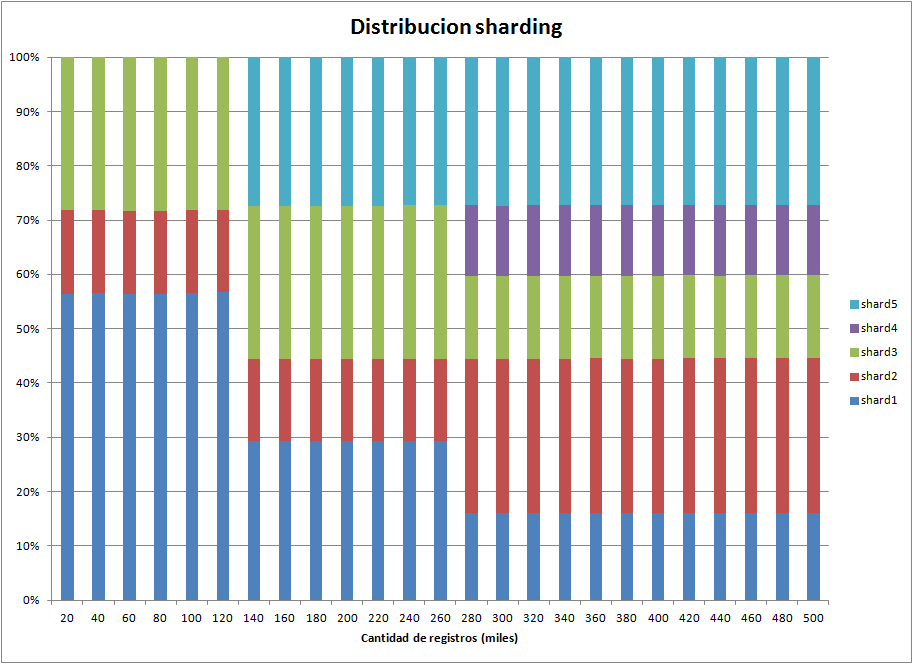
\includegraphics[width=165mm]{../mediciones/sharding_simple.png}
\caption{Porcentaje de distribucion entre los shards usando un
indice simple en base al codigo postal.}
\end{figure}

\begin{figure}[H]
\centering
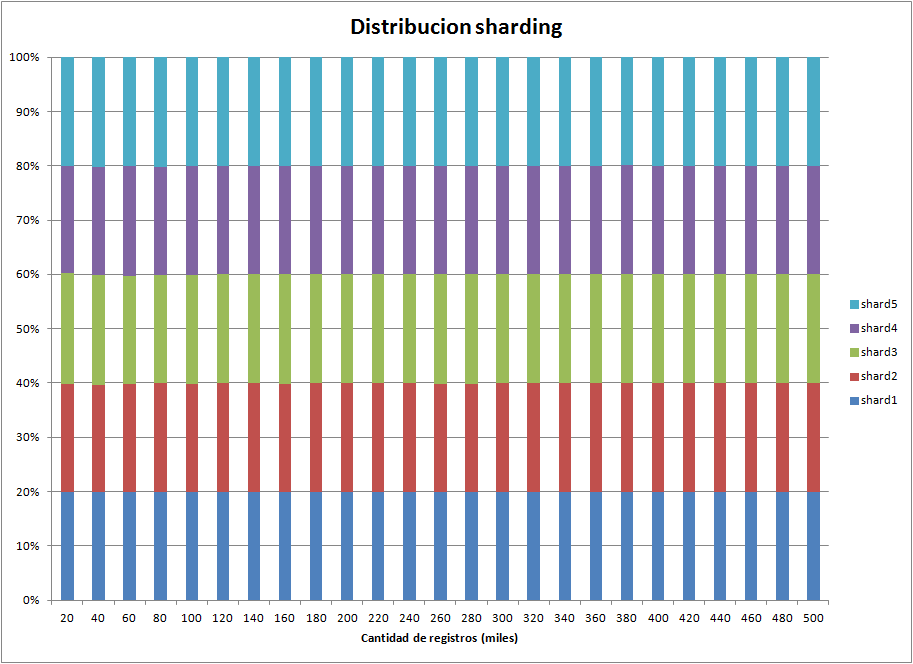
\includegraphics[width=165mm]{../mediciones/sharding_hashed.png}
\caption{Porcentaje de distribucion entre los shards usando un
indice hasheado en base al \_id}
\end{figure}



\newpage
\section{Otras base de datos NoSql.}


Base de datos key-value, usando el motor redis.
Redis permite el uso de namespaces (tener varios "diccionarios", la terminología de redis para esto sería "multiple databases"), lo cual hace el diseño más prolijo y simple.

Usar map-reduce en redis no es algo built-in ni estandar, pero investigamos y es posible, por
    ejemplo, integrarlo con Hadoop.

Parte1:
    1a:
        En redis hay un comando SCAN que permite iterar las claves.
        Con esto podemos iterar un diccionario de empleados, donde en cada
            value hay una lista de datos de cada cliente que atendió.
        Entonces se puede iterar las claves una por una y quedarse con las que
            tienen algun cliente mayor de edad.
    1b:
        Usando SCAN se puede iterar las claves de un diccionario
        articulos -> ventas. Mediante codigo se buscan las claves que tengan
        |ventas| maximo.

    1c:
        Idem usando SCAN. Si tenemos un diccionario sector -> [empleados], es cuestion
            de iterar y mediante código buscar cuando |empleados|==3

    1d:
        Un diccionario empleado -> [sectores]. Idem 1c usando SCAN.

    1e:
        Diccionario cliente  -> [compras]. Idem 1c, pero ordenando mediante |compras|.

    1f:
        Esta consulta ya es un poco más compleja, hay varios enfoques posibles.
        Uno es mantener las cosas simples y directamente usar un diccionario
            edad -> cantidadDeCompras. Por ser tan específico, es un diccionario
            que sólo sirve para esta consulta, con lo cual estamos agregando
            un costo de mantenimiento extra a la DB sólo por una query.
        Otra opción es valerse de map reduce y usar alguno de los otros diccionarios,
            como el de 1a. Como ventaja, la consulta es simple y no hace falta crear un diccionario extra
            solo por esta consulta.


Parte 2:
    Asumimos que se crea un id único para las disposiciones, podría ser un hash de sus datos o
        la combinación (numeroBoja, paginaInicial, PaginaFinal) que asumimos que identifica
        univocamente a la disposicion. Entonces se tiene un diccionario id -> disposicion.

    Las resoluciones por map-reduce son prácticamente iguales a las versiones hechas en mongodb
        ya que la entrada de la función map es practicamente la misma.

Parte 3:
    TODO: primero habría que hacerlo en mongodb jaja.



\newpage
\section{Conclusiones}


Nos encontramos con varias soluciones para resolver el problema. Fueron muy valiosas las discuciones de ideas sobre diseños en el DER. También nos percatamos de la complejidad escondida que tienen los diseños, y como algo que parece simple puede ser muy complejo.
Es muy importante invertir tiempo en el diseño para simplificar las consultas y en general el modelo en la base de datos. Tanto fue así, que con el modelo propuesto en el DER logramos soluciones a las consultas bastantes simples, incluso sin necesidad de Triggers.

Para la resolución de las consultas surgieron distintas opciones. La consulta HistorialLicencia se realizo inicialmente con una subquery. Luego transformamos esta subquery en una Vista. Para finalizar realizamos la consulta generando una nueva tabla de Participantes en un siniestro. Esto generó un profundo aprendizage en el uso de los Triggers.

En la generación de los datos tuvimos algunos inconvenientes para carga tablas con muchas FKs. Muchas de las cuales fueron creadas manualmente y con poca cantidad de registros. También nos hubiera gustado generar casos mas complejos, pero por la cantidad de depenedencias se hacia dificultoso.






\end{document}
